\section{Gradient Boosting Decision Trees}

We have also experimented with \gls{gbdt} for predicting indoor locations. For evaluating the performance of the models, we use \gls{mpe}.%For evaluating the algorithm, we have used the regular \gls{gbdt} implementation from Kaggle and \gls{dart}.

\subsection{Gradient Boosting Decision Trees}
Initially, we have tested the \gls{gbdt} algorithm on the data provided by the feature engineering phase. Several tests were conducted to find the optimal number of estimators and learning rate. This resulted in the most optimal model performing as shown in \textbf{\autoref{fig:light_gbm1}}, which has 50000 number of estimators and 0.1 learning rate.

\begin{figure}[H]
    \centering
    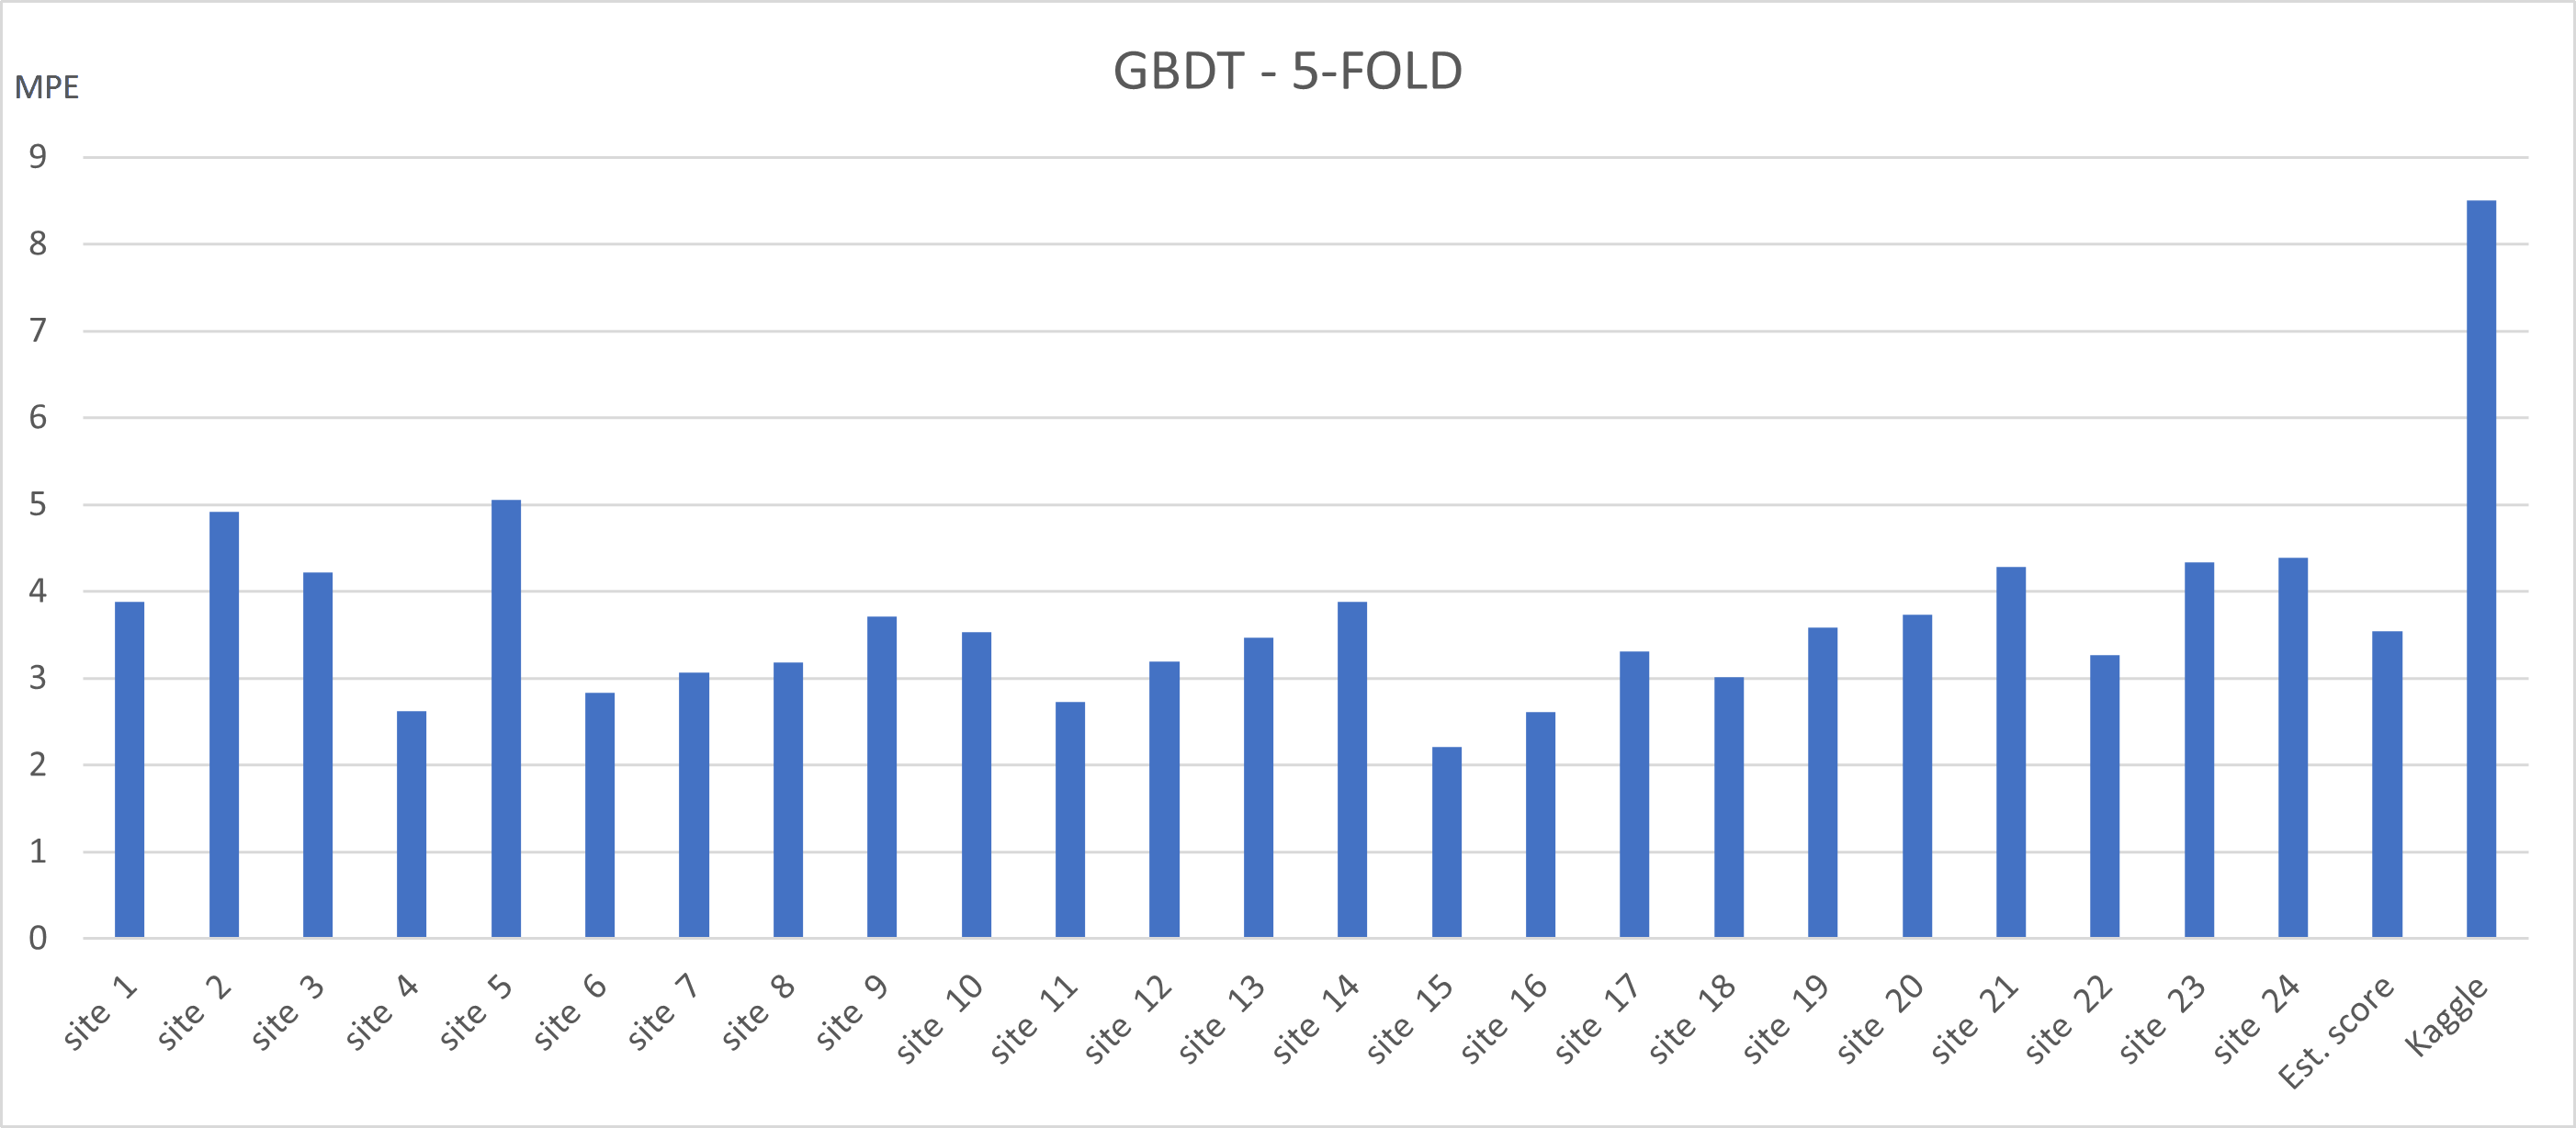
\includegraphics[scale=0.6]{Images/Experiments/lightgbm/GBDT-5.png}
    \caption{\gls{mpe} results for \gls{gbdt} for the different sites during training, the overall mean estimated score for all of the sites, and lastly the final score from Indoor Navigation \& Location competition on the test set.}
    \label{fig:light_gbm1}
\end{figure}

\textbf{\autoref{fig:light_gbm1}} displays the \gls{mpe} for the different sites from the training data individually as denoted on the x-axis. Thereafter, the mean of \gls{mpe} for all the training data is displayed marked in the figure as \textit{Est. Score}. The last column denotes the result from Indoor Navigation \& Location competition and displays the \gls{mpe} calculated by the competition from the prediction, we make on the provided test data.

We believe a reason for the huge difference between the training data and test data could be overfitting. To combat this, we tried to use the \gls{dart} algorithm instead.

\subsection{Dropouts meet Multiple Additive Regression Trees}

As mentioned in \textbf{\autoref{sec:problemsmachinelearning}}, an issue for a lot of machine learning models is overfitting, as seen in \textbf{\autoref{sec:problemsmachinelearning}}. To combat the issue of overfitting for \gls{gbdt}, \gls{dart} was used. This algorithm was presented in the paper \cite{dart} by K. V. Rashmi and Ran Gilad-Bachrach, and it applies the dropout technique to gradient boosting regression trees. This does not eliminate overfitting in its entirety, but reduces it to a certain extent.\cite{dart}

Dropout is a technique used most commonly for neural networks to reduce overfitting, which is explained in \textbf{\autoref{sec:over_underfit}}. The technique is concerned with randomly dropping units with their connections from the neural network during the training phase. The purpose is to remove units before their start to overspecialise. The dropout technique, as presented in the paper \cite{dropout}, has proved to increase performance of neural networks for supervised learning tasks, since it reduces overfitting.

In each iteration, the different trees are assigned a probability to be dropped. At the bare minimum, at least a single tree is dropped in each iteration. In the paper \cite{dart}, they use the \textit{binomial-plus-one} technique to select which trees to drop and if no trees are selected, then one tree is randomly chosen to be dropped.

Based on these papers, there exists an implementation of \gls{dart} in LightGBM. We tried to apply this instead of the regular \gls{gbdt}, and managed to get the results shown in \textbf{\autoref{fig:light_gbm2}}.

\begin{figure}[H]
    \centering
    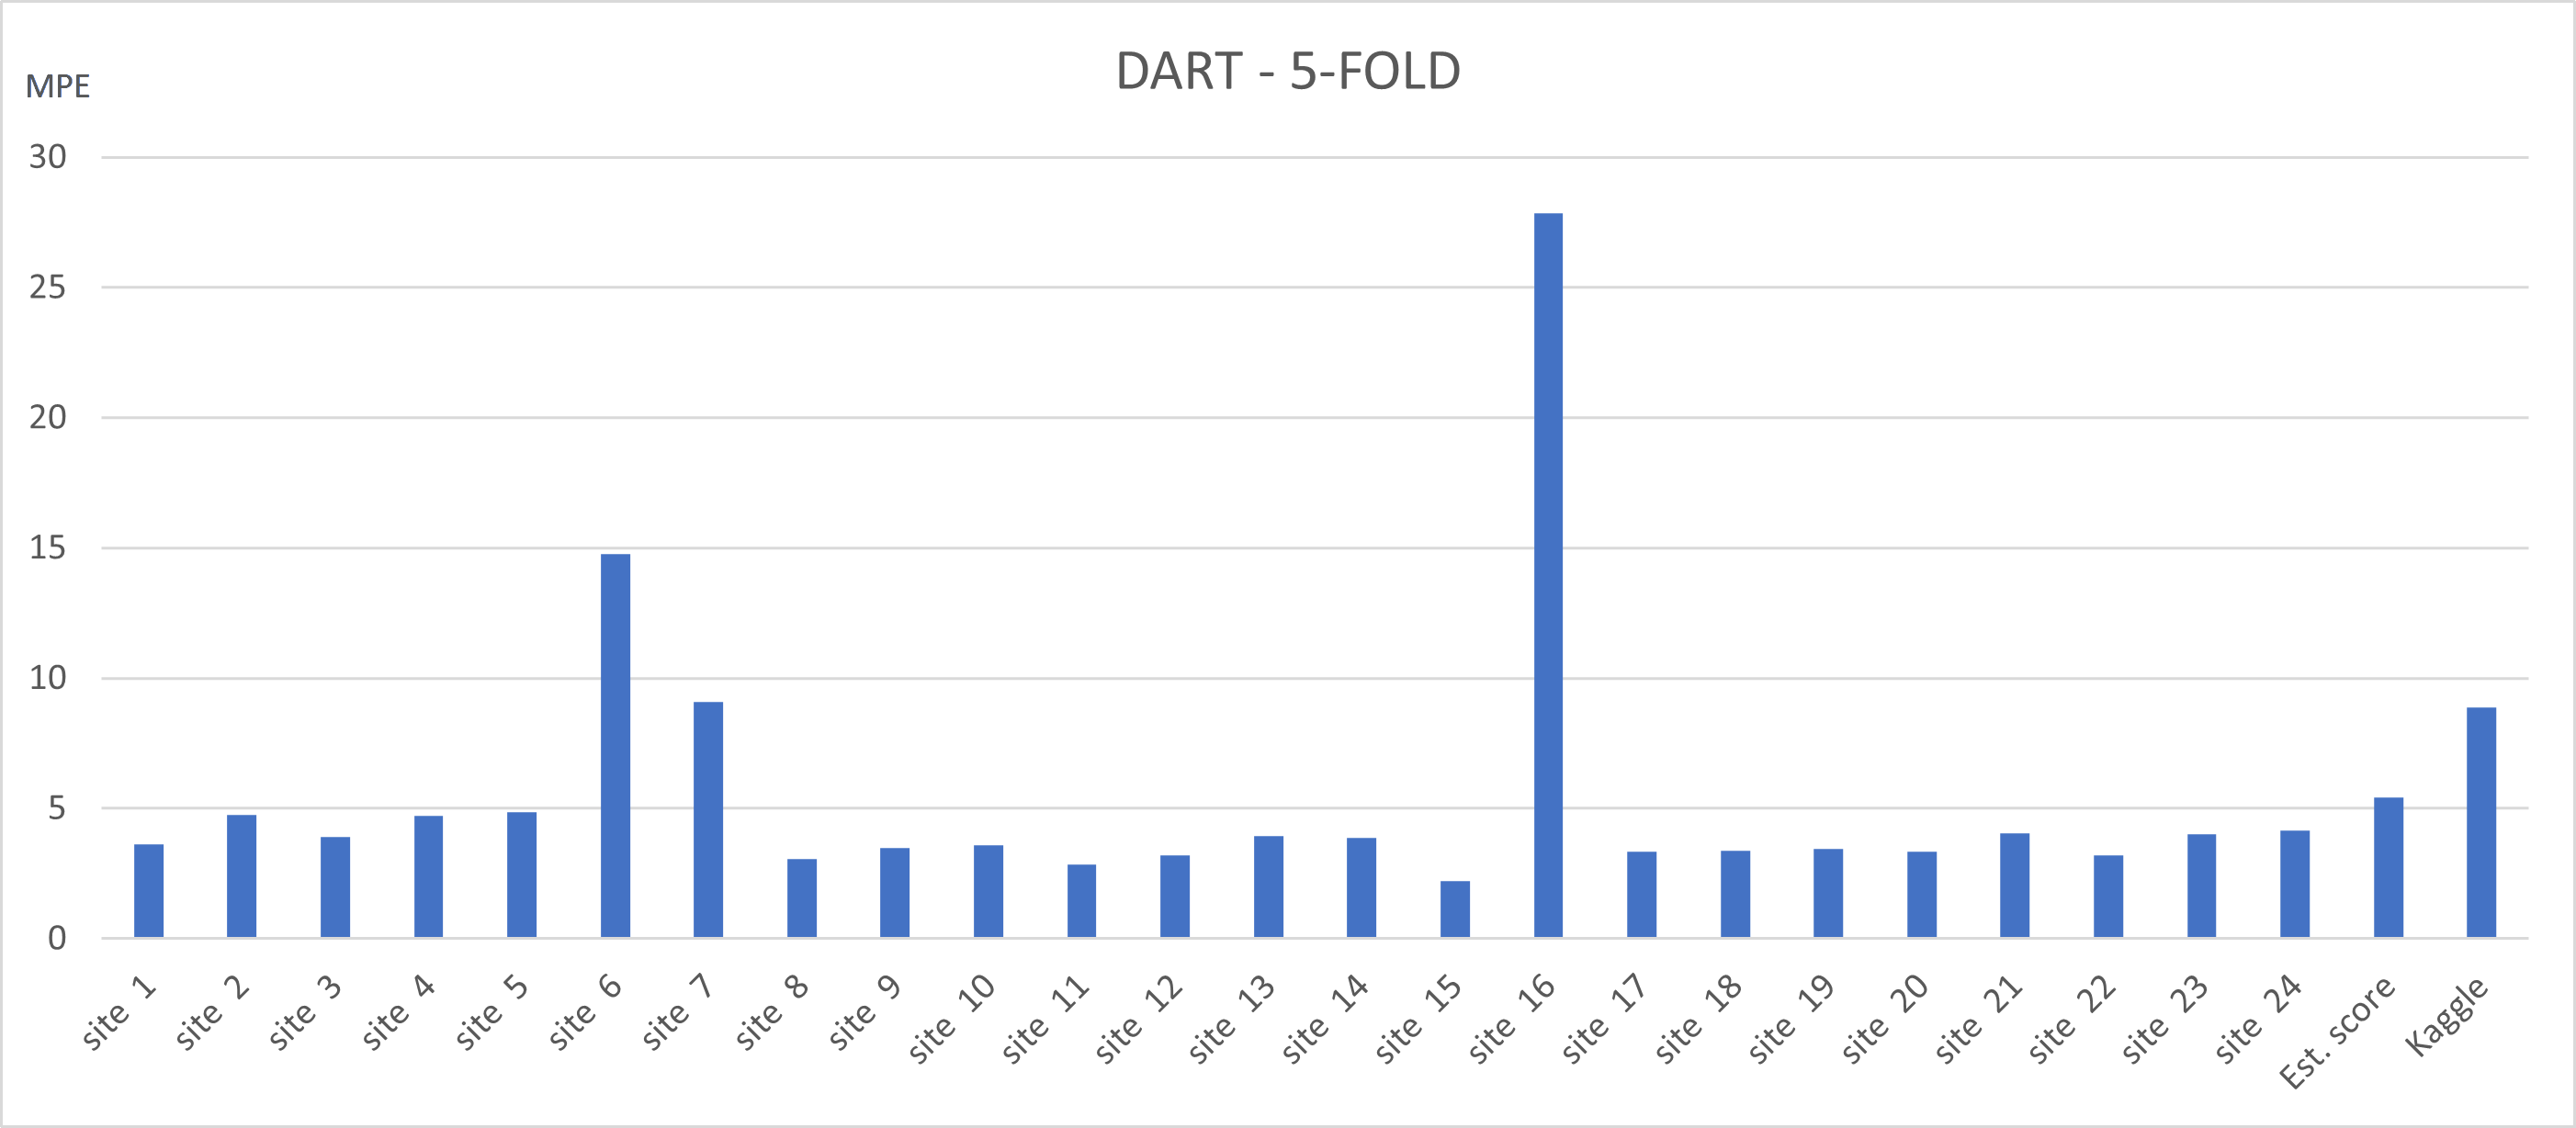
\includegraphics[scale=0.6]{Images/Experiments/lightgbm/DART_5.png}
    \caption{Mean position error results for \gls{dart} displaying the different site scores during training and lastly the overall estimated score and the final score from Kaggle on the test set.}
    \label{fig:light_gbm2}
\end{figure}

Applying the \gls{dart} algorithm instead, did not impact the result for most of the training data and test data, but it did worsened the performance of two sites especially (site 6 and site 16). Since these two sites are also present in the test data and the overall score is not impacted, a level of overfitting should have been reduced. When comparing the mean \gls{mpe} to the Kaggle score, the \gls{dart} implementation has a smaller difference than the \gls{gbdt} implementation. Even though the Kaggle score is similar our expectation to the \gls{dart} implementation are worse. With these results, we expect that the \gls{dart} algorithm combats overfitting more efficiently and has a better potential for further testing, but due to time constraints, we might not be able to keep testing the \gls{dart} implementation.

\begin{figure}[H]
    \centering
    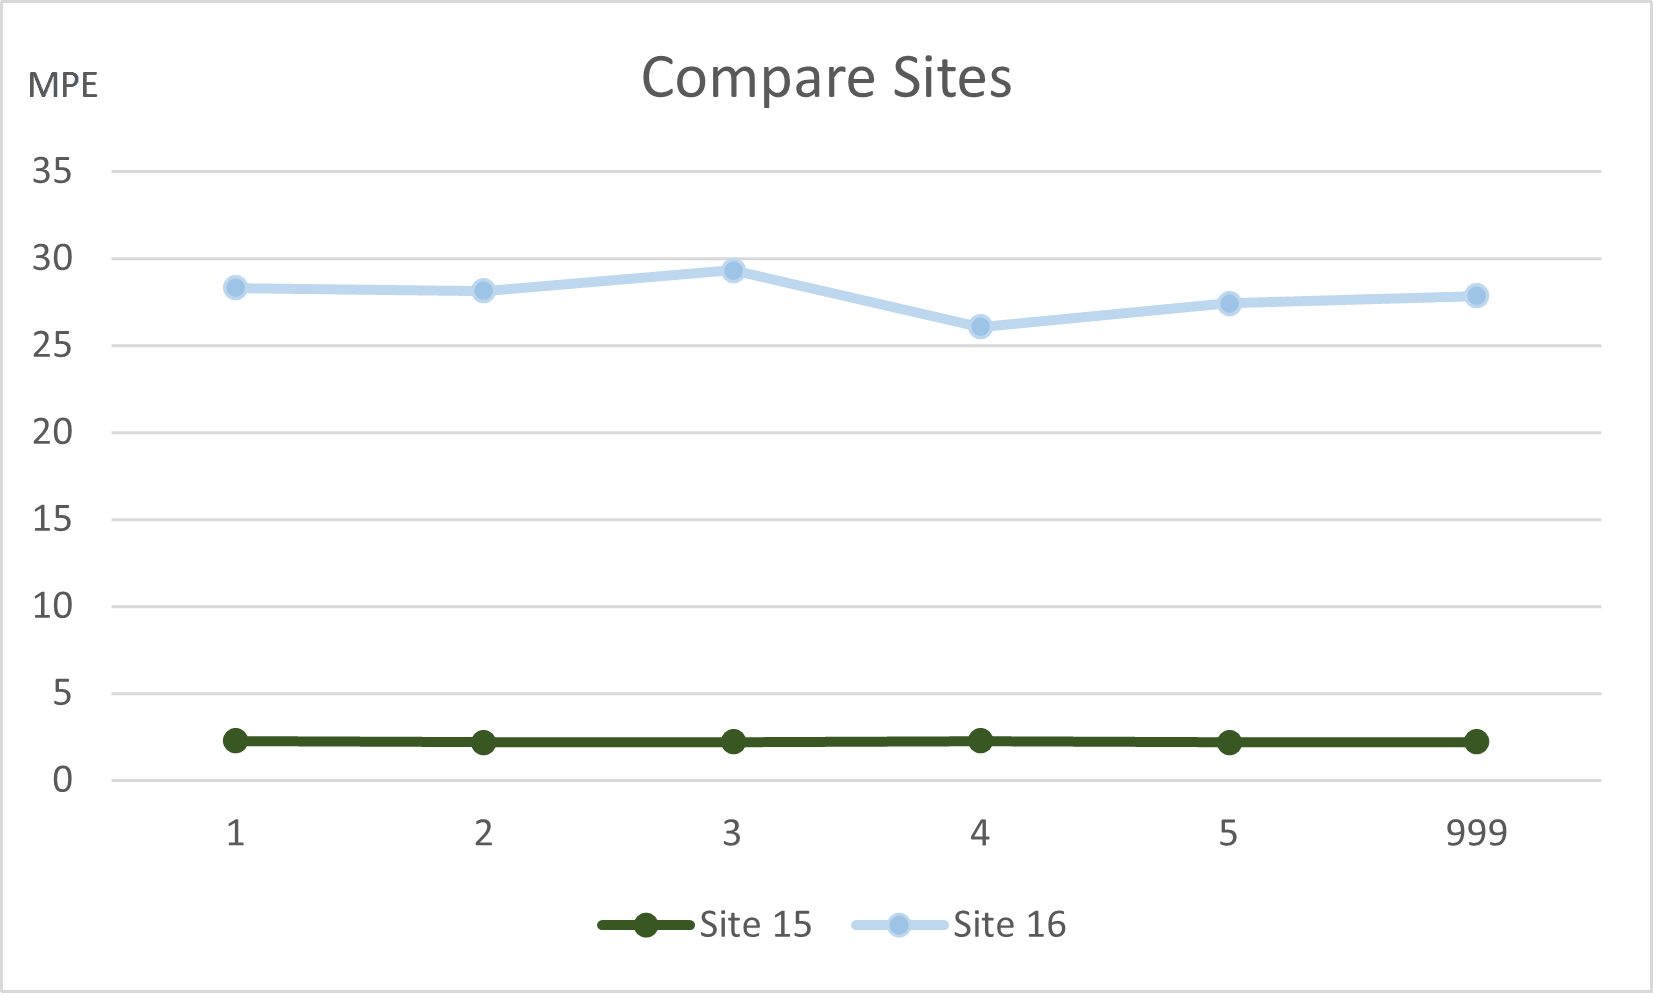
\includegraphics[scale=0.6]{Images/Experiments/lightgbm/compare.png}
    \caption{\gls{mpe} for the two sites at each fold, and lastly the mean of \gls{mpe} for all five folds, which is denoted as 999 instead of the fold number.}
    \label{fig:light_gbm3}
\end{figure}

\textbf{\autoref{fig:light_gbm3}} displays a closer view into the \gls{mpe} for each fold for \textit{site 16} and \textit{site 15}. Here, it is clear to see that the model does not perform better through the different folds, but that \textit{site 16} performs a lot worse than the other sites. 

Even though \gls{dart} does not significantly outperform \gls{gbdt} in the results, we imagine a larger potential with the right hyper-parameters. With the observation of the smaller overfitting and the sites in which we can get better performance, this algorithm could be a great option for our hybrid solution. A problem, however, with the \gls{dart} implementation is that it is much more resource demanding and therefore it is more time consuming to find the right hyper-parameters. Due to the slow progress using \gls{dart}, we, however, have decided to use \gls{gbdt} as the possible hybrid component because of the similar performance reached and requirement of resources in other parts of the system.